\RequirePackage{luatex85}
\documentclass[tikz]{standalone}
\begin{document}
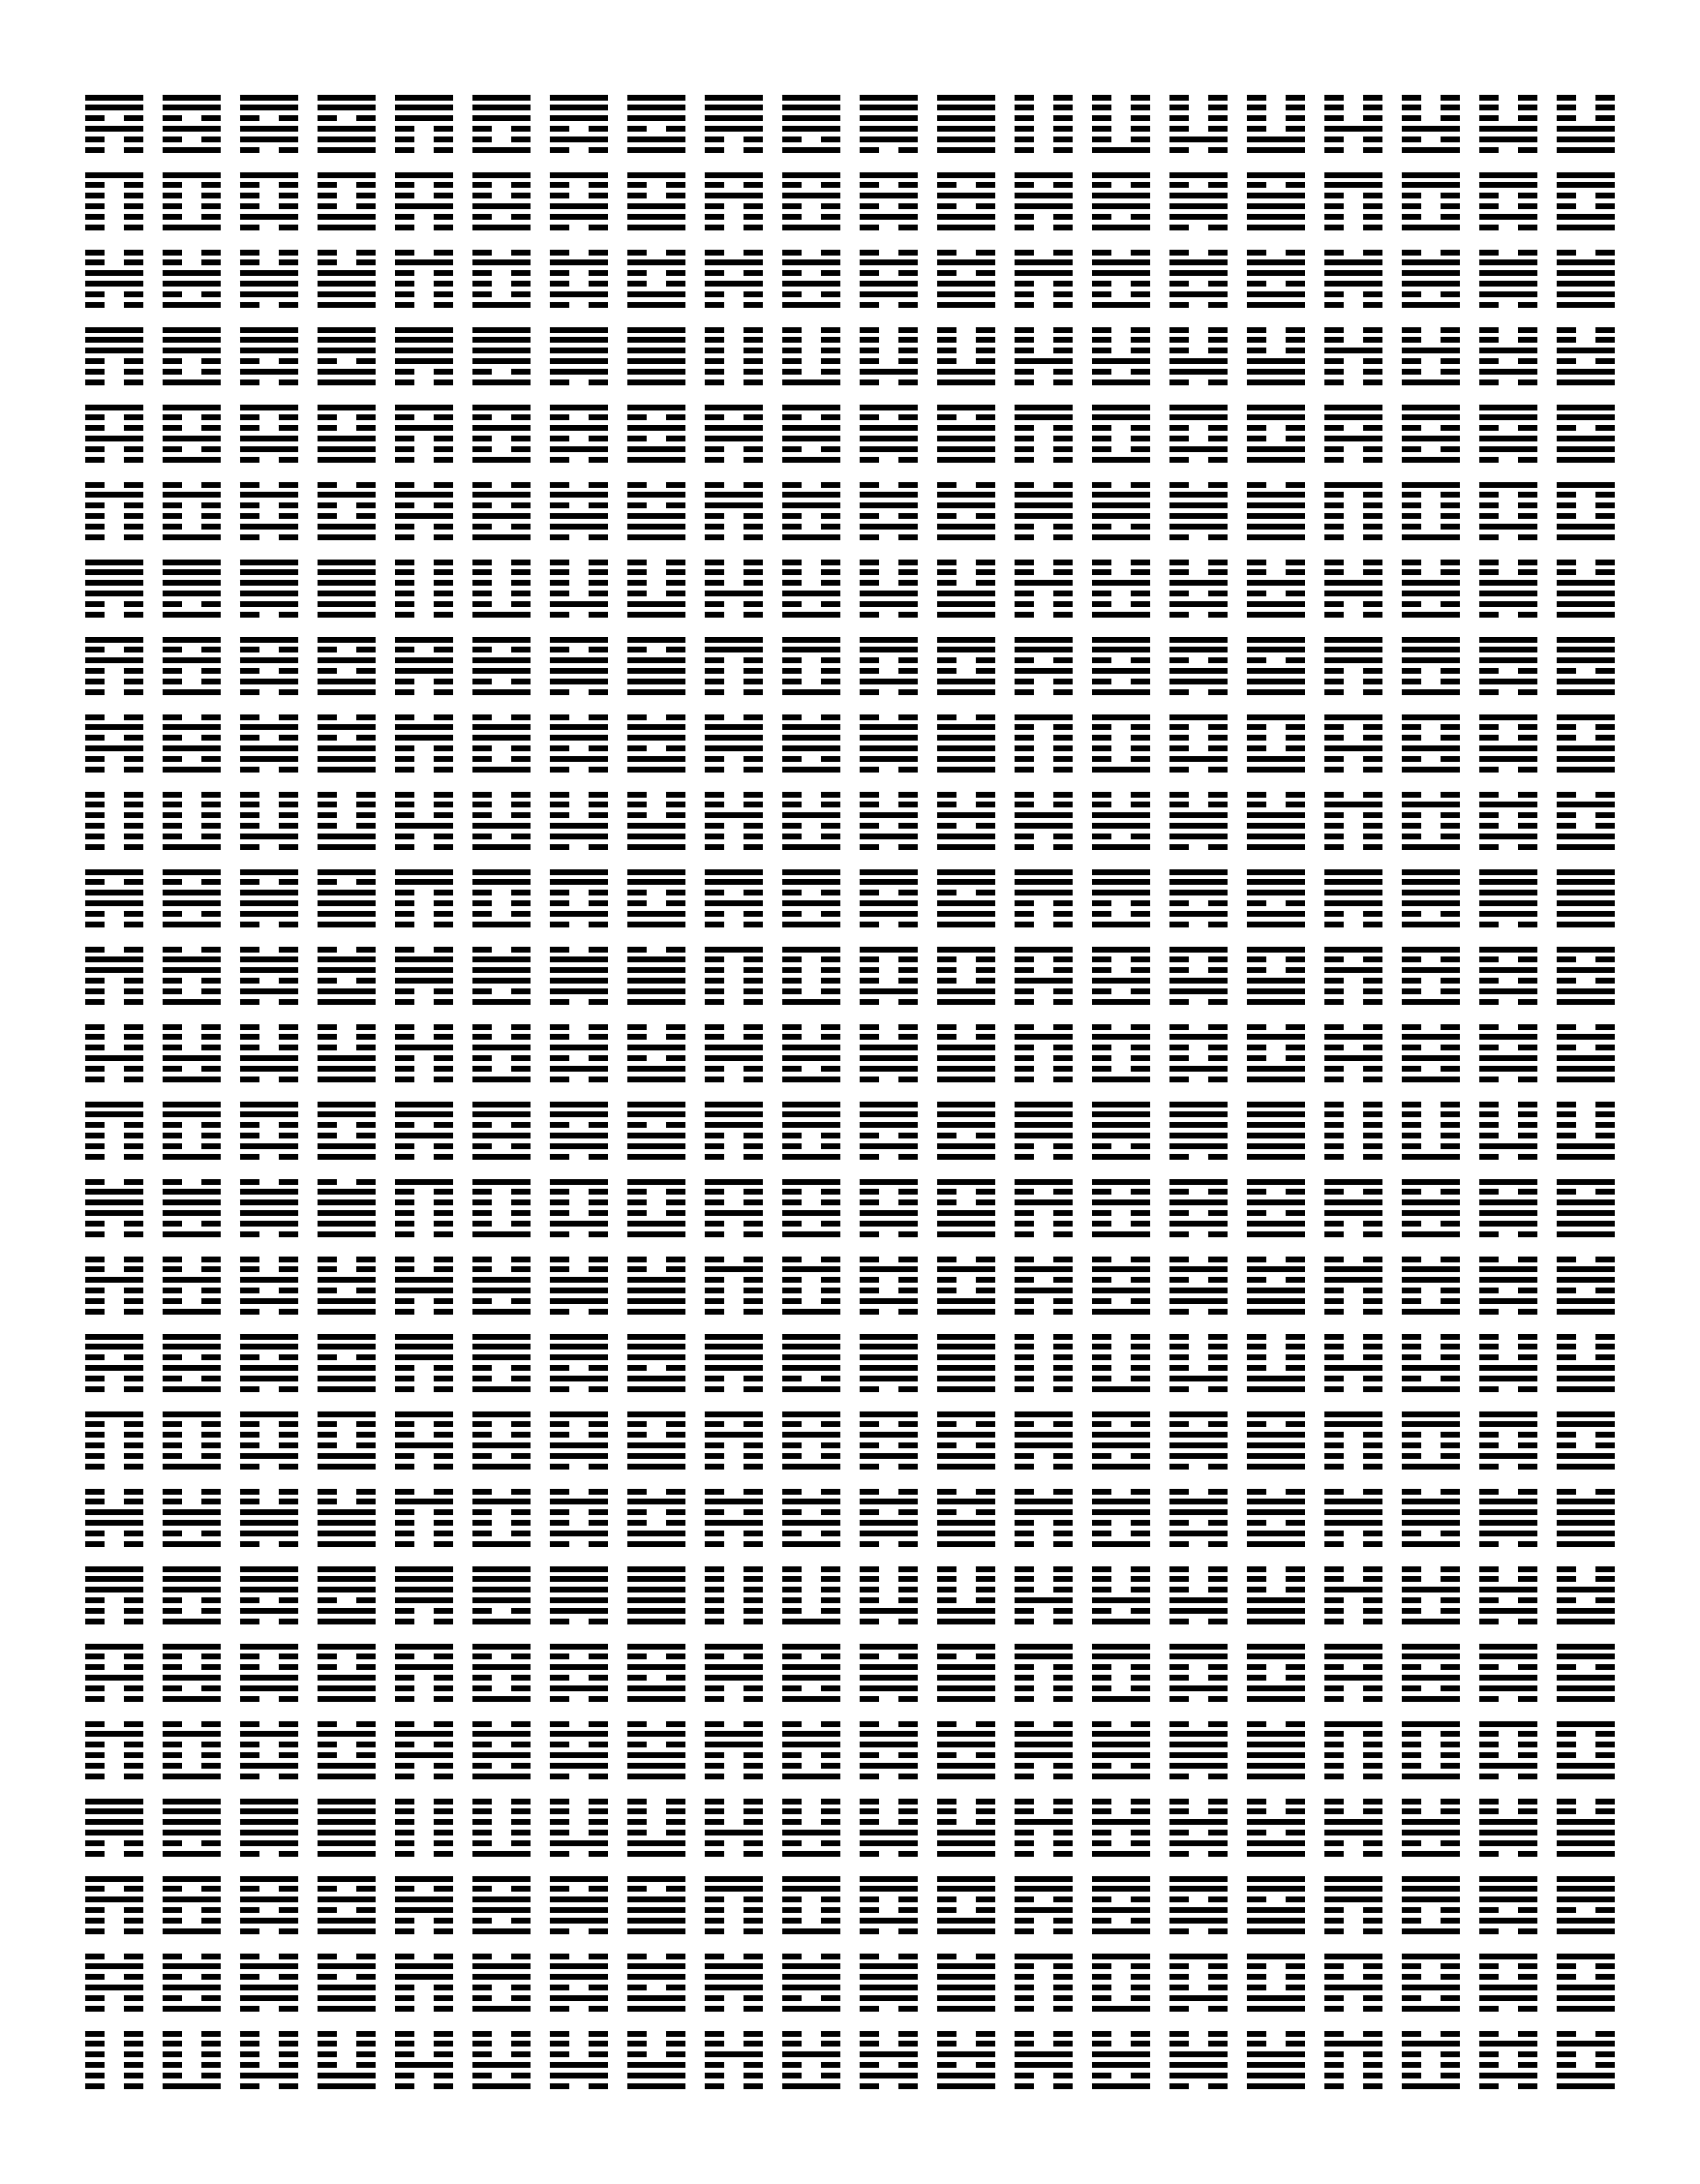
\begin{tikzpicture}
% 0.03in = \barwidth
[line width=0.03in]
\clip (0,0) rectangle (8.5in,11in);
\foreach \row in {0,...,25}{ % 25 = 26-1 = \numrows-1
\foreach \col in {0,...,19}{ % 19 = 20-1 = \numcols-1
\foreach \bar in {0,...,5}{
	% 0.3in = \leftmargin
	% 0.4in = 0.1in+0.3in = \xsep+\barlen
	% 0.365in = 0.35in+0.5*0.03in = \bottommargin+0.5*\barwidth
	% 0.054in = 0.03in+0.024in = \barwidth+\barsep
	% 0.4in = 6*0.03in+5*0.024in+0.1in = 6*\barwidth+5*\barsep+\ysep
	\draw ({0.3in+\col*0.4in}, {0.365in+\bar*0.054in+\row*0.4in}) coordinate (xy);
	% 20 = \numcols
	\pgfmathtruncatemacro\barval{mod(floor(mod(\col+20*\row,64)/2^\bar),2)}
	\ifnum\barval=0
	\draw (xy) -- ++(right:0.1in) ++(right:0.1in) -- ++(right:0.1in);
	\else\draw (xy) -- ++(right:0.3in);\fi
	}}}
\end{tikzpicture}
\end{document}